%%%%%%%%%%%%%%%%%%%%%%%%%%%%%%%%%%%%%%%%%%%%%%%%%%%%%%%%%%%%%%%%%%%%%%%%%%
%%%%%%%%%%%%   CHAPTER 3   %%%%%%%%%%%%%%%%%%%%%%%%%%%%%%%%%%%%%%%%%%%%%%%%
%%%%%%%%%%%%%%%%%%%%%%%%%%%%%%%%%%%%%%%%%%%%%%%%%%%%%%%%%%%%%%%%%%%%%%%%%%
\chapter{The Proposed Algorithm}
\label{chap:algorithm}

This chapter deals with the choice of the algorithm and the software optimizations done to it. The requirements of the algorithm are listed. Various components of the algorithm are explained. Software optimizations done to the algorithm to improve the execution time are explained. The final optimized version of the algorithm is presented and elaborated.


%%%%%%%%%%%%%%%%%%%%%%%%%%%%%%%%%%%%%
%%%%%%%%%%%%%%%%%%%%%%%%%%%%%%%%%%%%%
%%%%%%%%%%%%   SECTION   %%%%%%%%%%%%
%%%%%%%%%%%%%%%%%%%%%%%%%%%%%%%%%%%%%
%%%%%%%%%%%%%%%%%%%%%%%%%%%%%%%%%%%%%
\section{Algorithm requirements}
\label{s:requirements}

A binocular stereovision, as discussed in the Chapter \ref{chap:backgroundandrelatedwork}, involves taking each pixel in an image (for example left image), finding the corresponding pixel in the other image (right image), and finding the shift of the pixel between images. Considering the assumptions made in the Section \ref{s:stereovision} and the architecture of Nema GPU, the algorithm has a set of requirements to produce a reliable DM:
\begin{enumerate}
    \item The variations in the image due to reflections need to be reduced. Light from distant light sources reflects off different points in the scene before reaching the left and the right cameras. This will result in variations in the images as illustrated in the Figure \ref{fig:reflection}. These variations need to be reduced.
    \item The noise and gain of each camera need to be accounted for and normalised. Though the physical properties of the camera like focal length and resolution are assumed to be same, the image sensor of each camera might vary in performance. This might result in a certain point in the scene seeming brighter, for example, in one of the cameras compared to another. Such differences in the left and right images need to be reduced.
    \item In order to ease the GPU implementation, the algorithm is preferred to operate on integer variables. Nema GPU has the data size of 32 bits and the normal GPU functionality produces results to be written to the frame buffer of the display (32-bit pixels). Hence, it is desirable that the algorithm also produces results in integer format.
    \item The algorithm must be easily translatable for GPU implementation. It should be compatible with the kernel structure discussed in the Chapter \ref{chap:backgroundandrelatedwork}.
    \item The algorithm needs to be optimised as much as possible for run-time prior to GPU implementation. In order to narrow down any reduction in performance due to GPU bottleneck, this is desirable.
\end{enumerate}

\begin{figure}
\begin{subfigure}{.5\textwidth}
  \centering
  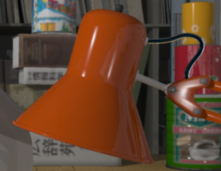
\includegraphics[width=.6\linewidth]{figures/reflectionleft}
  \caption{Left camera image}
  \label{fig:sfrl}
\end{subfigure}%
\begin{subfigure}{.5\textwidth}
  \centering
  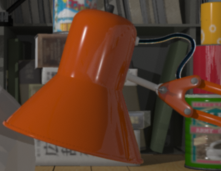
\includegraphics[width=.6\linewidth]{figures/reflectionright}
  \caption{Right camera image}
  \label{fig:sfrr}
\end{subfigure}
\caption{Reflection of light from distant light source}
\label{fig:reflection}
\end{figure}



%%%%%%%%%%%%%%%%%%%%%%%%%%%%%%%%%%%%%
%%%%%%%%%%%%%%%%%%%%%%%%%%%%%%%%%%%%%
%%%%%%%%%%%%   SECTION   %%%%%%%%%%%%
%%%%%%%%%%%%%%%%%%%%%%%%%%%%%%%%%%%%%
%%%%%%%%%%%%%%%%%%%%%%%%%%%%%%%%%%%%%
\section{Algorithm}
\label{s:algorithm}

The algorithm chosen for the evaluation addresses the stated requirements. The noise and gain of the camera are normalised by taking the census transform of both images. In order to reduce the variations in the image, the morphological transformation is applied. The chosen algorithm operates on integer variables. The compliance of the next two requirements will be evident as this chapter progresses. The algorithm chosen operates on monochrome versions of the images. The algorithm is split into two parts: Preprocessing and DM calculation as shown in the Figure \ref{fig:algorithmstructure}.

\begin{figure}
    \center
    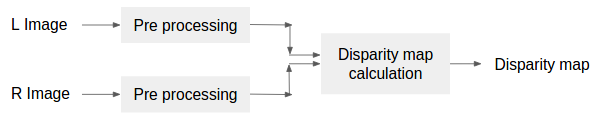
\includegraphics[width=.8\linewidth]{figures/algorithm_structure}
    \caption{Algorithm structure.}
    \label{fig:algorithmstructure}
\end{figure}
%

%%%%%%%%%%%%%%%%%%%%%%%%%
%%%%%   SUB-SECTION   %%%
%%%%%%%%%%%%%%%%%%%%%%%%%
%%%%%%%%%%%%%%%%%%%%%%%%%
\subsection{Preprocessing}
\label{s:algorithm:preprocessing}

The preprocessing stage involves reducing noise and variations between the two cameras. Variations in the images due to reflections is tackled by the morphological opening of each of the images \cite{Rosli2014}. The morphological opening consists of two parts: Morphological erosion, and Morphological dilation. Morphological erosion by any structure assigns the lowest value in the structure to the centre pixel. For a 3x3 square structure, morphological erosion at a pixel involves assigning the lowest value among the neighbouring pixels to that pixel as shown in the Figure \ref{fig:morphologicalerosion}.

 \begin{figure}
    \center
    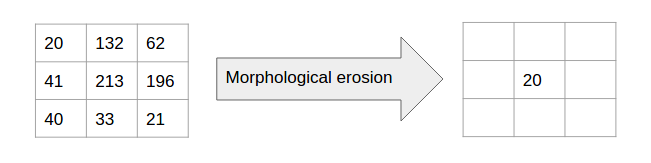
\includegraphics[width=120mm]{figures/Morphological_erosion}
    \caption{Morphologial erosion.}
    \label{fig:morphologicalerosion}
\end{figure}


Similarly, morphological dilation by any structure assigns the highest value in the structure to the centre pixel. For a 3x3 square structure, morphological dilation at a pixel involves assigning the highest value among the neighbouring pixels to that pixel as shown in the Figure \ref{fig:morphologicaldilation}.

 \begin{figure}
    \center
    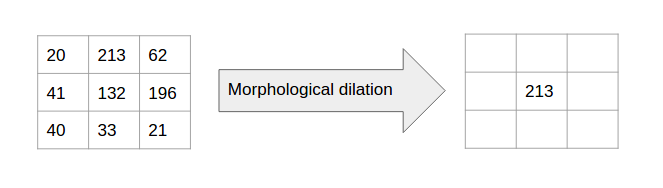
\includegraphics[width=120mm]{figures/Morphological_dilation}
    \caption{Morphologial dilation.}
    \label{fig:morphologicaldilation}
\end{figure}

Morphological erosion followed by dilation is called morphological opening and it is known to reduce white blobs in the image \cite{Rosli2014}. Thus, effects due to reflection on each image are reduced consequently reducing the variations between them.

The normalisation of the gain and the noise of cameras is done by census transform \cite{Zabih1994}\cite{young_ki_baik_fast_2006}. Census transform of a pixel P(x,y) is given by the Equation \ref{eqn:censustransform}.

\begin{equation}
  C(P) = \underset{[i,j]\in W}{\otimes} {\xi (P(x,y),P(x+i,y+j))} 
  \label{eqn:censustransform}
\end{equation}

Here $\bigotimes$ denotes concatenation, W denotes window of operation around P and $\xi$ is given by 

\[ \xi (P(x,y),P(x+i,y+j)) =
  \begin{cases}
    1       & \quad \text{if } P(x,y)>P(x+i,y+j)\\
    0  & \quad \text{if } \text{otherwise}\\
  \end{cases}
\]

\begin{figure}[!htbp]
    \center
    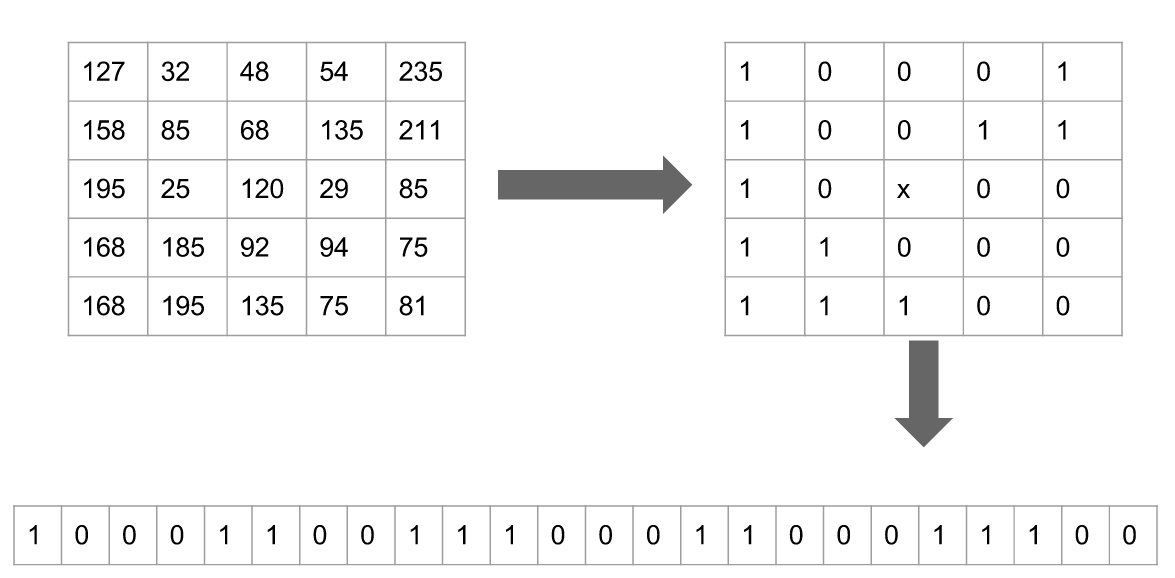
\includegraphics[width=.8\linewidth]{figures/Censustransform_example}
    \caption{Census transform example for 5x5 window.}
    \label{fig:censusexample}
\end{figure}

An example of a census transform for a 5x5 window around a pixel is as shown in the Figure \ref{fig:censusexample}. A census transformed image is invariant under changes in gain and bias \cite{young_ki_baik_fast_2006}. Hence, it can be used for normalisation of gains of both cameras.

%%%%%%%%%%%%%%%%%%%%%%%%%
%%%%%   SUB-SECTION   %%%
%%%%%%%%%%%%%%%%%%%%%%%%%
%%%%%%%%%%%%%%%%%%%%%%%%%
\subsection{Disparity Map calculation}
\label{s:algorithm:dmcalculation}

For the purpose of DM calculation, Sum of Hamming Distances (SHD) algorithm is used. This algorithm is chosen as it has the best speed performance in parallel architecture like FPGA or GPU \cite{GyorgyTamasBiroKaroly-Agoston2015}. It is a window based comparison technique. Here a window of pixels around each pixel in one image (left) is compared for a match in the other image (right). Generally, window based comparison algorithm assume all pixels in the window have a similar disparity value \cite{Hamzah2015}. However, this is not true. Hence, there is a poor performance in the regions where there is a large change in disparity values within a window. SHD algorithm is known to be robust against this issue \cite{Hamzah2015}. SHD between two census transformed pixels is calculated by XORing each bit of all the pixels within a window of a particular size around the pixels, and summing the result up. Mathematically SHD at a pixel x,y can be expressed as shown in the Equation \ref{eqn:shd}.

\begin{equation}
  SHD(x,y,D) = \underset{[i,j]\in W}{\sum} {{\sum_{\substack{bits}}}XORbitwise\big(P(x+i,y+j),Q(x+i-D,y+j)\big)} 
  \label{eqn:shd}
\end{equation}

Here P is the reference image(left image), Q is the target image(right image), W denotes window of operation and D denotes the disparity level.\\
Disparity of a particular pixel
\begin{equation}
  DM(x,y) = \underset{D\in [a..b]}{argmin}{\big(SHD(x,y,D)\big)}
  \label{eqn:dm}
\end{equation}

where D is the range of disparity levels with a and b as minimum and maximum values respectively.

In the current thesis, 3x3 square structure is used for morphological opening, 11x11 window is used for census transform and 13x13 window is used for DM calculation. The disparity levels range from 0 to 100. The choice of these values is explained in Chapter 4.


%%%%%%%%%%%%%%%%%%%%%%%%%%%%%%%%%%%%%
%%%%%%%%%%%%%%%%%%%%%%%%%%%%%%%%%%%%%
%%%%%%%%%%%%   SECTION   %%%%%%%%%%%%
%%%%%%%%%%%%%%%%%%%%%%%%%%%%%%%%%%%%%
%%%%%%%%%%%%%%%%%%%%%%%%%%%%%%%%%%%%%
\section{Optimizations}
\label{sec:optimizations}

The algorithm is implemented in C\textbackslash C++ and run on various PCs. The first version of the algorithm is implemented in Matlab to ensure its functionality. Subsequent versions are implemented in C++. The png++ library is used for image input and output. Various optimizations done on the initial C++ version to improve the execution time are discussed in this section. The results of each optimization on different platforms is presented in the next chapter.

\subsection{Datastructure optimization}
\label{s:optimizations:dsoptimization}

\begin{figure}[!htbp]
    \center
    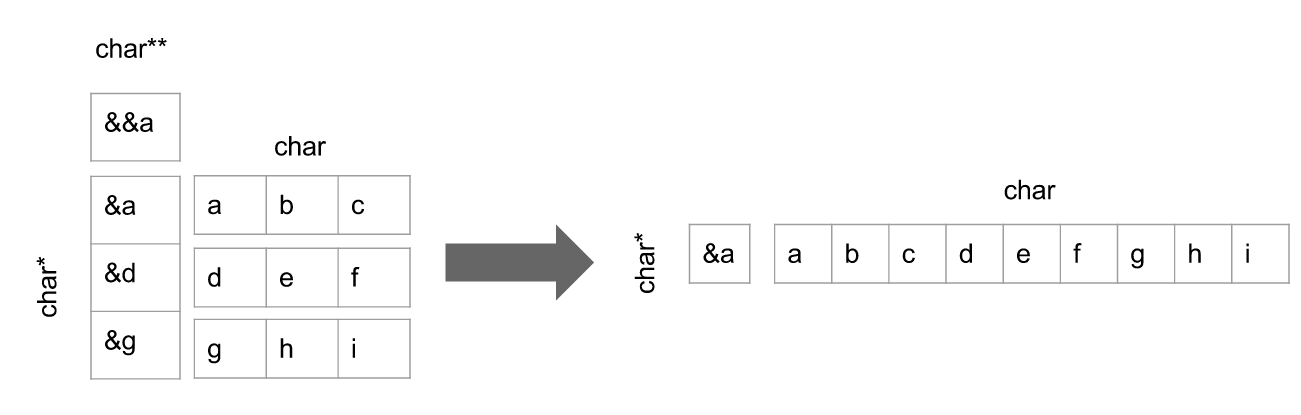
\includegraphics[width=.8\linewidth]{figures/dsoptimization}
    \caption{Datastructure optimization.}
    \label{fig:dsoptimization}
\end{figure}

The initial C++ version of the algorithm stores unprocessed images in 2D arrays. The elements of the array are referenced by a char** pointer. Manipulating and dereferencing a char** pointer gives a char* pointer or the row of an element in the array. The char* pointer, in turn, can be manipulated and dereferenced to reveal an element of the array. It is clear that in order to access a particular pixel of the image (element of the array) two levels of dereferencing needs to be done. This can be reduced to a single level dereferencing by replacing the 2D arrays by pseudo-2D arrays \cite{Souli2007}. Now the data structure of an unprocessed image is a 1D array. Now every pixel can be directly accessed from the memory using char* datatype. The same optimization is done for different versions of the image reducing the number of dereferences and hence improving the run-time performance. This optimization is illustrated in the Figure \ref{fig:dsoptimization} for a 3x3 array.

\subsection{Multithreading}
\label{s:optimizations:multithreading}

The DM calculation part of the algorithm chosen is parallelizable. This is because the calculation of DM at any pixel is independent of the DM calculation at another pixel. Many implementation platforms have a multi-core capability. This advantage provided by the platform can be utilised in order to speed up the algorithm \cite{threadcpp}. The images are split into four sections and the DM calculation at each part of the image is issued as a different thread. This allows parallel execution of the algorithm and leads to improvement in run-time performance.

\subsection{Invariant code motion}
\label{s:optimizations:invariantcodemotion}

\begin{figure}[!htbp]
    \center
    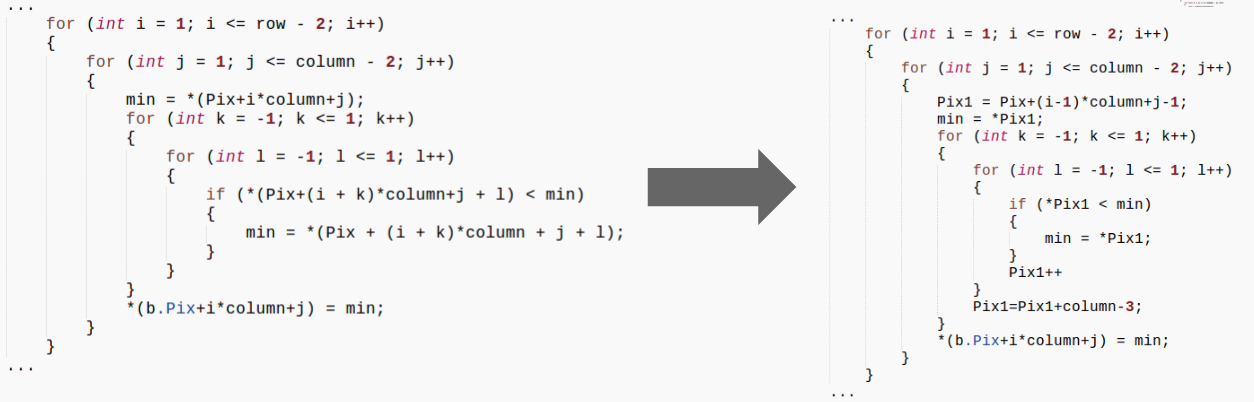
\includegraphics[width=\linewidth]{figures/icmoptimization}
    \caption{Invariant code motion optimization.}
    \label{fig:icmoptimization}
\end{figure}

DM calculation in the algorithm involves multiple loops with pointer manipulation and dereferencing inside the innermost loop. This involves calculation of address of a pixel every iteration involving multiple operations. Since most of the calculations happen between consecutive pixels, if the address of the current pixel is stored and incremented, it can be used to access the required pixel in the next iteration \cite{Aho2006}. One other way of seeing this is that iteration variables of the outer loop remain invariant in the innermost loop and hence the calculations involving can be moved outside the loop and stored. This optimization works well if the hardware has enough registers to store the newly created variables. In case, the hardware does not contain enough registers the variables might get spilled. The case of insufficient registers could also happen due to the execution of multiple threads of the same function, creating a need for more variables. Invariant code motion optimization is illustrated in the Figure \ref{fig:icmoptimization}. Here one can notice that by creating a variable Pix1 in loop 2, one can save a lot of calculations on Pix in loop 4. This is replaced by a simple increment on Pix1.

\subsection{SIMD}
\label{s:optimizations:simd}
Census transform with an 11x11 window for each pixel results in a 120-bit value. This is stored in two long integers(64 bit each). During the DM calculation, XOR operation is performed on these data between two images. One can notice that the same operation is performed on multiple variables(two long integers) for each pixel. This can be accelerated using the vectorization techniques offered by the processor \cite{Siewert2009}. The resulting implementation produces just one operation(128 bit XOR) for each pixel instead of two. Acceleration obtained by this SIMD(single instruction multiple data) operation is studied.

\subsection{Store and reuse of XOR values}
\label{s:optimizations:xoroptimization}

\begin{figure}[!htbp]
    \center
    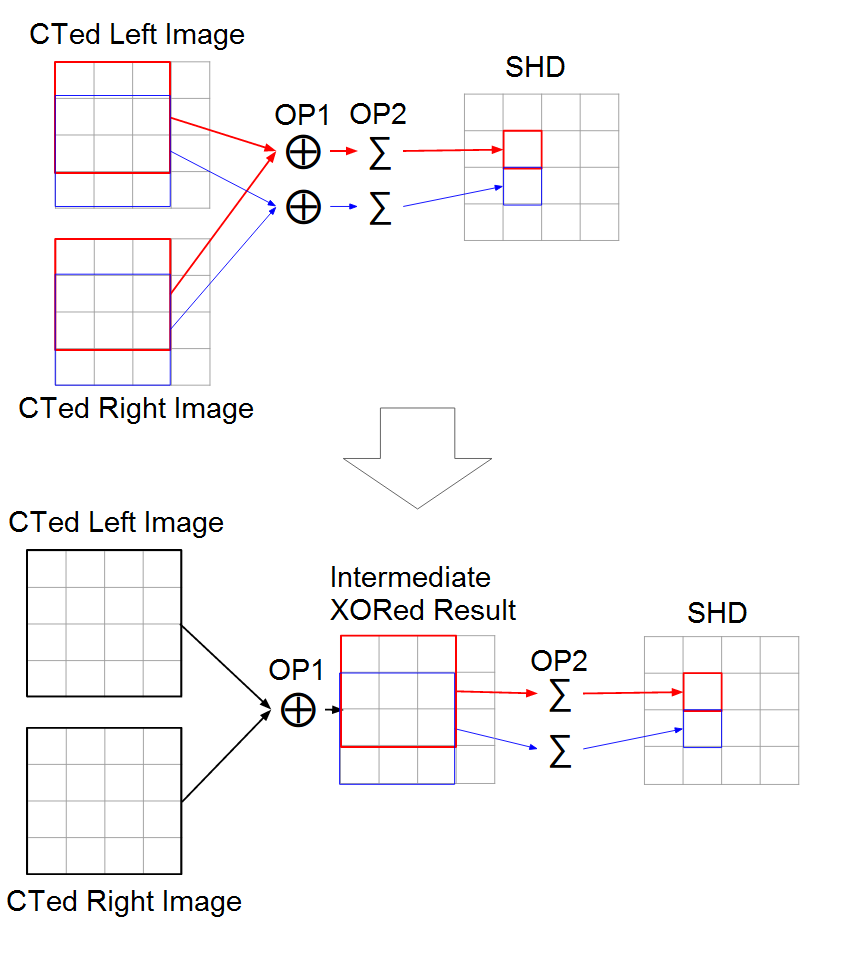
\includegraphics[width=.8\linewidth]{figures/xoroptimization}
    \caption{Storage and reuse of XOR values.}
    \label{fig:xoroptimization}
\end{figure}

The formula for SHD calculation is given in the Equation \ref{eqn:shd}. For an arbitrary position (x,y), the sum of bits in bitwise XOR is performed for all elements in the window around (x,y). Consider this as OP1. They are then summed up together to give the SHD at (x,y). Consider this as OP2. Moving on to the next position (x+1,y) OP1 needs to be performed on all elements in the window around (x+1,y). However, it is noticeable that the window is just shifted by one position, and most of the elements in the window of (x,y) are also present in the window of (x+1,y). Hence, most of the OP1 calculations are repeated. The implementation of the Equation \ref{eqn:shd} can be optimized by performing OP1 for all elements in the images for a particular disparity value and storing the results. These results for each element can be reused while performing OP2 at different positions to obtain SHD of the position. This optimization naturally leads to the lesser amount of calculations with a trade-off requiring more memory. Optimization involving storage and reuse of XOR values is illustrated in the Figure \ref{fig:xoroptimization}.

\subsection{Store and reuse of partial SHD values}
\label{s:optimizations:shdoptimization}

\begin{figure}[!htbp]
    \center
    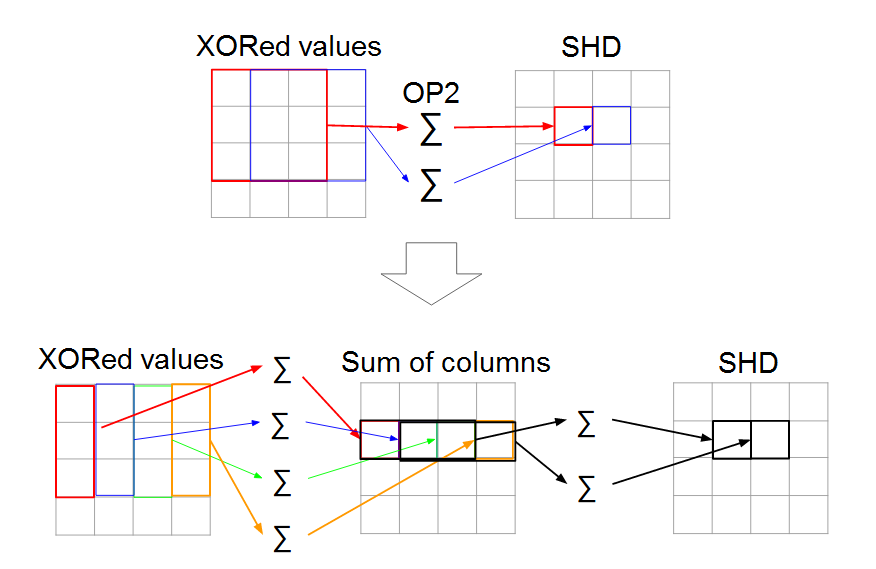
\includegraphics[width=.8\linewidth]{figures/parsumoptimization}
    \caption{Storage and reuse of partial SHD values.}
    \label{fig:parsumoptimization}
\end{figure}

The formula for SHD calculation is given in the Equation \ref{eqn:shd}. Consider the definition of OP2 provided in the Section \ref{s:optimizations:xoroptimization}. OP2 which is basically the sum of all elements within a window can be sequentially performed in many ways. One of the ways is first performing the sum of all columns and then performing the sum of results. It is noticeable that between positions (x,y) and (x+1,y), all but one column of the windows are the same. Hence, if the sum of columns are stored they can be reused across windows. For each element (x,y) the column vector of size same as the height of the window is summed up and stored. Then the required column vectors for each position (x,y) are summed up to provide the sum of elements of the window. This reuse of sum of column vectors reduces the number of calculations required for calculating the SHD at any position (x,y).  Optimization involving storage and reuse of partial SHD values is illustrated in the Figure \ref{fig:parsumoptimization}.

%%%%%%%%%%%%%%%%%%%%%%%%%%%%%%%%%%%%%
%%%%%%%%%%%%%%%%%%%%%%%%%%%%%%%%%%%%%
%%%%%%%%%%%%   SECTION   %%%%%%%%%%%%
%%%%%%%%%%%%%%%%%%%%%%%%%%%%%%%%%%%%%
%%%%%%%%%%%%%%%%%%%%%%%%%%%%%%%%%%%%%
\section{Optimized DM algorithm}
\label{sec:optdmalgo}

\begin{figure}
    \center
    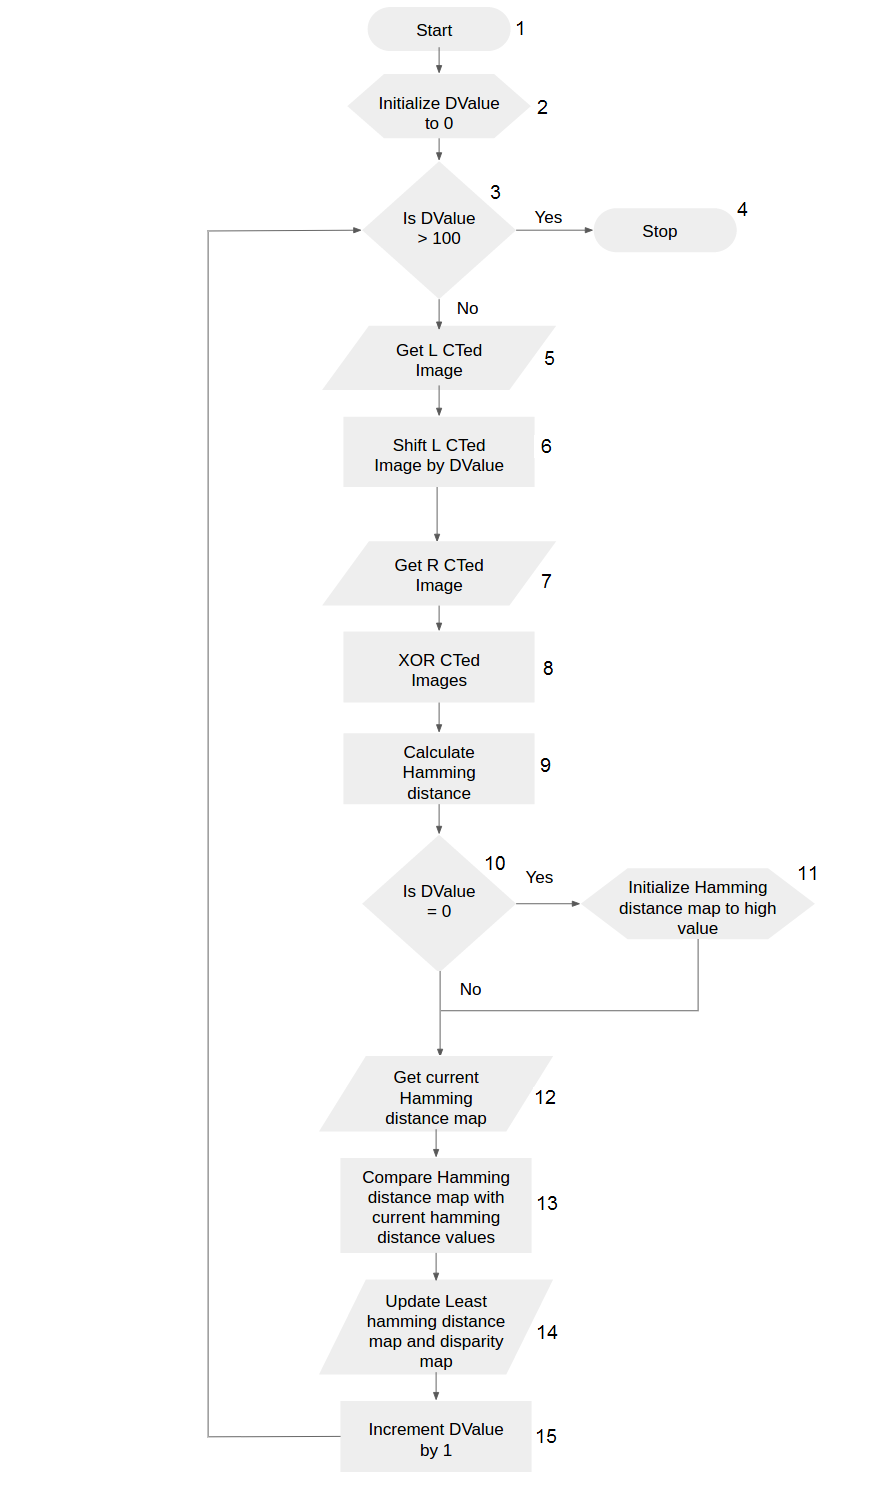
\includegraphics[width=.8\linewidth]{figures/shdalgorithm}
    \caption{Optimized version of DM algorithm.}
    \label{fig:shdalgorithm}
\end{figure}

The DM algorithm resulting after applying all the optimizations is shown in the Figure \ref{fig:shdalgorithm}. The flowchart shown is for the calculation of DM for a single frame after preprocessing is done. In the figure, the algorithm is shown to loop for 101 iterations, each iteration for a disparity value (DValue). DValue is initialized with 0 (2). The census transformed images are taken as inputs (5,7). The left image is shifted by the DValue (6). OP1 and OP2 from the Figure \ref{fig:xoroptimization} is done for the images (8,9). In the first iteration, a hamming distance map with very high values corresponding to each pixel is initialized. This map is compared with the hamming distances obtained from 9 for each pixel (13). The pixels of the hamming distance map are updated in case the new hamming distance from 9 is lower than the current value (14). The corresponding pixels in the DM are also updated with the current DValue (14). The DValue is incremented and the loop is iterated for the entire range of DValues (15,3). The updated DM once the loop is complete gives the required disparity values at each pixel.

%%%%%%%%%%%%%%%%%%%%%%%%%%%%%%%%%%%%%
%%%%%%%%%%%%%%%%%%%%%%%%%%%%%%%%%%%%%
%%%%%%%%%%%%   SECTION   %%%%%%%%%%%%
%%%%%%%%%%%%%%%%%%%%%%%%%%%%%%%%%%%%%
%%%%%%%%%%%%%%%%%%%%%%%%%%%%%%%%%%%%%
\section{Summary}
\label{sec:summary3}

The chapter discussed on the proposed algorithm and various optimizations done to it. The optimizations included software optimizations as shown in the Subsections \ref{s:optimizations:dsoptimization}, \ref{s:optimizations:multithreading}, \ref{s:optimizations:invariantcodemotion} and \ref{s:optimizations:simd}, and algorithm modifications as shown in the Subsections \ref{s:optimizations:xoroptimization} and \ref{s:optimizations:shdoptimization}. The resulting algorithm for DM creation was discussed. The effects of these optimizations and the effect of parameter change in the algorithm is discussed in the next chapter.